%----------------------------------------------------------------------------------------
% TWEEDEGRAADSVERGELIJKINGEN. Alle opgaven zijn eigen werk.
%
% Opbouw: Probleem, Start, leerstof, en op een nieuwe pagina de Opdrachten en Test jezelf (geen Koppel in de 2de graad).
% Labels van dit hoofdstuk beginnen met h3-.
% Pakketten: dit hoofdstuk staat in pakket 2-5. Verschillen: ontbinden met de oplossingen a(x - x1)(x - x2) (4-5),
% het bewijs van de formule met de discriminant, de som en het product van de oplossingen en bikwadratische vergelijkingen (5).
%----------------------------------------------------------------------------------------

\mychapter{3}{Tweedegraadsvergelijkingen}

\begin{probleem}
\vspace{-1mm}\naast{Een rechthoekig grasveld is $20$ m lang en $15$ m breed. Rondom komt een grindpad dat overal even breed is. Er is grind voor $200$ m$^2$, en het moet allemaal op het pad. Hoe breed wordt het pad? Proberen lukt maar half: met een pad van $2$ m heb je $156$ m$^2$ grind nodig, met $3$ m al $246$ m$^2$. Het antwoord ligt ertussen, maar waar precies?}{\begin{tikzpicture}[x=.14cm,y=.14cm,font=\scriptsize]
  \fill[black!12] (-2.5,-2.5) rectangle (22.5,17.5);
  \draw[grijs] (-2.5,-2.5) rectangle (22.5,17.5);
  \fill[accent!25] (0,0) rectangle (20,15);
  \draw[accent,thick] (0,0) rectangle (20,15);
  \node at (10,7.5) {gras};
  \node[below] at (10,0) {$20$ m};
  \node[left] at (0,7.5) {$15$ m};
  \draw[inkt,<->] (20,10) -- (22.5,10) node[right] {$x$};
\end{tikzpicture}}
\end{probleem}

\lkr{Leerplan \pakketnaam: LPD \alleenvoor{2}{27}\alleenvoor{3}{28}\alleenvoor{4,5}{32} (tweedegraadsvergelijkingen grafisch oplossen) en LPD \alleenvoor{2}{28}\alleenvoor{3}{29}\alleenvoor{4,5}{33} (algebraïsch oplossen: ontbinden in factoren en de discriminant, met de wenken over $ax^2 + bx = 0$, $ax^2 + c = 0$ en het kritisch controleren van de oplossingen in een context). \alleenvoor{4,5}{ Ontbinden met de oplossingen hoort bij de wenk over de vorm $a(x - x_1)(x - x_2)$ (het voorschrift met de nulwaarden staat in hoofdstuk 1).}\alleenvoor{5}{ De som en het product van de oplossingen volgen een wenk bij LPD 33, de bikwadratische vergelijkingen een extra; het servicedocument voor 5 uur maakt beide verplicht. Het bewijs van de formule met de discriminant hoort bij B1. }\alleenvoor{4,5}{ Het aantal oplossingen bespreken met een parameter (een extra bij LPD 33) staat in de opdrachten en in hoofdstuk 4.} Voorkennis: hoofdstuk 1 en 2, de merkwaardige producten en het buiten haakjes brengen uit de 1ste graad, en vierkantswortels uit Reële getallen. De som-productmethode is een techniek om te ontbinden (een leerinhoud van het doel), geen apart doel; laat ze weg als de klas ze moeilijk vindt, want de discriminant werkt altijd. Het probleem komt terug in voorbeeld~\ref{vb:h3-terug}.}

In hoofdstuk 2 zag je dat de fontein ergens in de vijver terechtkomt, maar waar precies, dat kon je nog niet berekenen. Dat is een nulwaarde: een $x$ waarvoor $-0,8x^2 + 3,2x + 0,4 = 0$. Zo'n vergelijking met een kwadraat heet een tweedegraadsvergelijking. In dit hoofdstuk leer je ze oplossen: eerst de eenvoudige gevallen, dan door te ontbinden in factoren, en tot slot met een formule die altijd werkt. Je ziet ook wat de oplossingen op de grafiek betekenen.

\begin{oefeningen}[Start]
\oef{h3-start-1}

\oef{h3-verken}
\end{oefeningen}

%========================================================================================
\section{Onvolledige vergelijkingen}

\subsection{Wat is een tweedegraadsvergelijking?}

Bij het grasveld noemen we de breedte van het pad $x$. Grasveld en pad samen vormen een rechthoek van $20 + 2x$ op $15 + 2x$. Trek je het gras af, dan houd je het pad over:
\[(20 + 2x)(15 + 2x) - 300 = 200.\]
Werk je de haakjes uit en breng je alles naar het linkerlid, dan krijg je $4x^2 + 70x - 200 = 0$. Zo'n vergelijking heeft een term in $x^2$, net als een tweedegraadsfunctie.

\begin{theorie}
Een \textbf{\textcolor{accent}{tweedegraadsvergelijking}} is een vergelijking die je kunt herleiden tot de vorm

\qquad $\formule{ax^2 + bx + c = 0}$ \qquad met $a \neq 0$.
\end{theorie}

De oplossingen van $ax^2 + bx + c = 0$ zijn de nulwaarden van de functie $f(x) = ax^2 + bx + c$. Op de grafiek zijn het de $x$-coördinaten van de snijpunten van de parabool met de $x$-as. Uit hoofdstuk 2 weet je dus al dat er twee, één of geen oplossingen kunnen zijn.

We beginnen met de vergelijkingen waarin $b$ of $c$ nul is. Die heten \textit{onvolledig}, en ze zijn snel opgelost.

\subsection{Zonder term in \texorpdfstring{$x$}{x}: \texorpdfstring{$ax^2 + c = 0$}{ax² + c = 0}}

Is $b = 0$, dan breng je de vergelijking in de vorm $x^2 = k$, zoals in het handboek Reële getallen. Is $k > 0$, dan zijn er twee oplossingen $\pm\sqrt k$. Is $k = 0$, dan is $x = 0$. Is $k < 0$, dan is er geen oplossing.

\voorbeeld{}{Los op: $3x^2 - 48 = 0$.\label{vb:h3-zonderb}}{%
\uitleg{Er is geen term in $x$. We maken $x^2$ vrij.}
\begin{stappen}
3x^2 = 48 & Tel $48$ op bij beide leden. \\
x^2 = 16 & Deel door $3$. \\
x = 4 \ \text{ of } \ x = -4 & $V = \{-4, 4\}$.
\end{stappen}}

\subsection{De product-nulregel}

Wanneer is een product nul? Neem $(x - 2)(x + 5)$. Vul je $x = 2$ in, dan is de eerste factor $0$, en $0$ maal eender welk getal is $0$. Vul je $x = -5$ in, dan is de tweede factor $0$. Zijn beide factoren verschillend van $0$, dan is hun product dat ook: $3 \cdot 7 \neq 0$, en $(-1) \cdot 0,5 \neq 0$.

\begin{theorie}
\begin{stelling}{Product-nulregel}
Een product is nul als en slechts als minstens een van de factoren nul is:

\qquad $\formule{A \cdot B = 0 \iff A = 0 \ \text{ of } \ B = 0}$.
\end{stelling}
\end{theorie}

Dat werkt alleen met $0$ in het rechterlid. Uit $A \cdot B = 6$ kun je niets besluiten over $A$ of $B$ apart: $2 \cdot 3 = 6$, maar ook $1 \cdot 6$ en $12 \cdot 0,5$.

\subsection{Zonder constante term: \texorpdfstring{$ax^2 + bx = 0$}{ax² + bx = 0}}

Is $c = 0$, dan zit $x$ in elke term. Breng $x$ buiten haakjes, en je hebt een product dat nul is.

\voorbeeld{}{Los op: $2x^2 - 6x = 0$.\label{vb:h3-zonderc}}{%
\uitleg{Elke term bevat $x$, en ook de factor $2$. We brengen $2x$ buiten haakjes en gebruiken de product-nulregel.}
\begin{stappen}
2x(x - 3) = 0 & $2x$ buiten haakjes. \\
2x = 0 \ \text{ of } \ x - 3 = 0 & De product-nulregel. \\
x = 0 \ \text{ of } \ x = 3 & $V = \{0, 3\}$.
\end{stappen}
Een veelgemaakte fout: beide leden delen door $x$. Dan krijg je $2x - 6 = 0$, dus alleen $x = 3$. De oplossing $x = 0$ ben je kwijt, want delen door $x$ mag niet als $x = 0$ kan zijn.}

\begin{oefeningen}
\oef{h3-productnul}

\oef{h3-onvolledig}
\end{oefeningen}

%========================================================================================
\section{Ontbinden in factoren}

\subsection{Merkwaardige producten}

De product-nulregel werkt ook als $b$ en $c$ niet nul zijn, als je het linkerlid kunt schrijven als een product. Dat heet \textit{ontbinden in factoren}. Soms herken je een merkwaardig product: $A^2 - 2AB + B^2 = (A - B)^2$ of $A^2 - B^2 = (A - B)(A + B)$.

\voorbeeld{}{Los op: $x^2 - 10x + 25 = 0$.\label{vb:h3-kwadraat}}{%
\naast{\uitleg{We herkennen $(x - 5)^2 = x^2 - 2 \cdot 5x + 25$.}
\begin{stappenvrij}{3.4cm}{5cm}
(x - 5)^2 = 0 & Een merkwaardig product. \\
x - 5 = 0 & Beide factoren zijn gelijk. \\
x = 5 & $V = \{5\}$.
\end{stappenvrij}
\textit{Er is maar één oplossing. Op de grafiek raakt de parabool $y = (x - 5)^2$ de $x$-as in haar top.}}{\begin{tikzpicture}[x=.4cm,y=.3cm]
  \rooster{-1}{1}{8}{-1}{1}{5}
  \parabool{1}{5}{0}{2.75}{7.25}
  \toppunt[below right]{5}{0}{}
\end{tikzpicture}}}

\subsection{De som-productmethode}

Wat als je geen merkwaardig product herkent, zoals bij $x^2 - x - 12$? Kijk eerst hoe zo'n drieterm ontstaat. Werk $(x + 2)(x + 3)$ uit: $x^2 + 3x + 2x + 6 = x^2 + 5x + 6$. Het getal voor $x$ is de som $2 + 3$, het getal achteraan is het product $2 \cdot 3$. Omgekeerd zoek je dus twee getallen met een gegeven som en product.

\voorbeeld{}{Los op: $x^2 - x - 12 = 0$.\label{vb:h3-somproduct}}{%
\uitleg{We zoeken twee getallen met product $-12$ en som $-1$. Het product is negatief, dus ze hebben een verschillend teken. We proberen de paren met product $-12$.}
\begin{stappen}
1 \cdot (-12),\ 2 \cdot (-6),\ 3 \cdot (-4),\ \ldots & Paren met product $-12$; som $-11$, $-4$, $-1$: gevonden. \\
(x + 3)(x - 4) = 0 & De getallen zijn $3$ en $-4$. \\
x + 3 = 0 \ \text{ of } \ x - 4 = 0 & De product-nulregel. \\
x = -3 \ \text{ of } \ x = 4 & $V = \{-3, 4\}$.
\end{stappen}
Controle: $(-3)^2 - (-3) - 12 = 9 + 3 - 12 = 0$ en $16 - 4 - 12 = 0$.}

\begin{werkwijze}
Zorg dat het getal voor $x^2$ gelijk is aan $1$ (deel eventueel beide leden erdoor). Zoek twee getallen $m$ en $n$ met $m \cdot n = c$ en $m + n = b$. Dan is $x^2 + bx + c = (x + m)(x + n)$, en de oplossingen zijn $-m$ en $-n$. Vind je zulke getallen niet snel, gebruik dan de discriminant (verderop).
\end{werkwijze}

\begin{oefeningen}
\oef{h3-ontbinden}
\end{oefeningen}

\subsection{Eerst herleiden op nul}

De product-nulregel werkt alleen met $0$ in het rechterlid. Staat er een ander getal, dan werk je eerst alles uit en breng je alles naar het linkerlid.

\voorbeeld{}{Los op: $(x + 1)(x - 3) = 5$.\label{vb:h3-herleid}}{%
\uitleg{Het rechterlid is niet $0$. Besluiten dat $x + 1 = 5$ of $x - 3 = 5$ is fout. We werken de haakjes uit en trekken $5$ af.}
\begin{stappen}
x^2 - 3x + x - 3 = 5 & Haakjes uitwerken. \\
x^2 - 2x - 8 = 0 & Alles naar het linkerlid. \\
(x - 4)(x + 2) = 0 & Product $-8$ en som $-2$: $-4$ en $2$. \\
x = 4 \ \text{ of } \ x = -2 & $V = \{-2, 4\}$.
\end{stappen}
Controle: $(4 + 1)(4 - 3) = 5 \cdot 1 = 5$ en $(-2 + 1)(-2 - 3) = (-1) \cdot (-5) = 5$.}

\begin{oefeningen}
\oef{h3-nul}
\end{oefeningen}

%========================================================================================
\section{De discriminant}

\subsection{Een vergelijking die niet ontbindt}

Probeer $x^2 - 4x + 1 = 0$ met de som-productmethode: je zoekt twee getallen met product $1$ en som $-4$. Met gehele getallen lukt dat niet. Toch snijdt de parabool $y = x^2 - 4x + 1$ de $x$-as twee keer: haar top $(2, -3)$ ligt onder de as en ze is naar boven geopend. Hoe vinden we die snijpunten?

Het idee komt uit hoofdstuk 2: schrijf het voorschrift in de topvorm. Dan staat de onbekende maar één keer in de vergelijking.

\voorbeeld{}{Los op: $x^2 - 4x + 1 = 0$.\label{vb:h3-topvorm}}{%
\naast{\uitleg{De top is $(2, -3)$, dus $x^2 - 4x + 1 = (x - 2)^2 - 3$. Dan maken we het kwadraat vrij, zoals bij $x^2 = k$.}
\begin{stappenvrij}{5.2cm}{3.3cm}
(x - 2)^2 - 3 = 0 & De topvorm. \\
(x - 2)^2 = 3 & Tel $3$ op. \\
x - 2 = \sqrt3 \ \text{ of } \ x - 2 = -\sqrt3 & Twee getallen hebben $3$ als kwadraat. \\
x = 2 + \sqrt3 \ \text{ of } \ x = 2 - \sqrt3 & Ongeveer $3,73$ en $0,27$.
\end{stappenvrij}}{\begin{tikzpicture}[x=.45cm,y=.35cm]
  \rooster{-1}{1}{5}{-4}{1}{4}
  \symas{2}{-4}{4}
  \parabool{1}{2}{-3}{-.6}{4.6}
  \toppunt[below]{2}{-3}{}
  \punt{3.732}{0}\punt{.268}{0}
\end{tikzpicture}}
De twee oplossingen liggen symmetrisch om de as $x = 2$, op een afstand $\sqrt3$ ervan.}

Dit werkt voor elke tweedegraadsvergelijking. Doe je dezelfde stappen met de letters $a$, $b$ en $c$, dan krijg je een formule die je meteen kunt gebruiken. Daarin speelt één getal de hoofdrol: het getal dat in de plaats van $3$ komt en onder het wortelteken staat.

\begin{theorie}
De \textbf{\textcolor{accent}{discriminant}} van $ax^2 + bx + c = 0$ is het getal

\qquad $\formule{D = b^2 - 4ac}$.

\begin{stelling}{Oplossingen van een tweedegraadsvergelijking}
\textbullet\ Als $\formule{D > 0}$, heeft $ax^2 + bx + c = 0$ twee oplossingen:

\qquad $\formule{x_1 = \dfrac{-b + \sqrt D}{2a}}$ \quad en \quad $\formule{x_2 = \dfrac{-b - \sqrt D}{2a}}$.

\textbullet\ Als $\formule{D = 0}$, is er één oplossing: $\formule{x = -\dfrac{b}{2a}}$.

\textbullet\ Als $\formule{D < 0}$, zijn er geen oplossingen.
\end{stelling}
\alleenvoor{5}{\begin{bewijs}
Deel beide leden door $a \neq 0$ en splits het kwadraat af, zoals in hoofdstuk 2:
\bewijsregel{x^2 + \frac ba x + \frac ca = 0 \iff \Bigl(x + \frac{b}{2a}\Bigr)^2 - \frac{b^2}{4a^2} + \frac ca = 0 \iff \Bigl(x + \frac{b}{2a}\Bigr)^2 = \frac{b^2 - 4ac}{4a^2} = \frac{D}{4a^2}.}
Het rechterlid heeft het teken van $D$, want $4a^2 > 0$. Er zijn drie gevallen.

\textbullet\ $D < 0$: het rechterlid is negatief, en een kwadraat is nooit negatief. Er is geen oplossing.

\textbullet\ $D = 0$: dan is $\bigl(x + \tfrac{b}{2a}\bigr)^2 = 0$, dus $x + \tfrac{b}{2a} = 0$ en $x = -\tfrac{b}{2a}$.

\textbullet\ $D > 0$: de vierkantswortels van $\tfrac{D}{4a^2}$ zijn $\pm\tfrac{\sqrt D}{2\abs{a}}$, dus
\bewijsregel{x + \frac{b}{2a} = \pm\frac{\sqrt D}{2\abs{a}} = \pm\frac{\sqrt D}{2a} \qquad\text{zodat}\qquad x = \frac{-b \pm \sqrt D}{2a}.}
(Het teken van $2a$ maakt niet uit, want er staat $\pm$.)
\end{bewijs}}
\end{theorie}

\alleenvoor{2,3,4}{We bewijzen de formule hier niet: het zijn dezelfde stappen als in het voorbeeld, maar met letters. }De formule zegt ook iets over de grafiek. De oplossingen liggen symmetrisch om de as $x = -\tfrac{b}{2a}$, op een afstand $\tfrac{\sqrt D}{2\abs{a}}$ ervan. Hoe groter $D$, hoe verder ze uit elkaar liggen. Is $D = 0$, dan vallen ze samen in de top.

\figuren{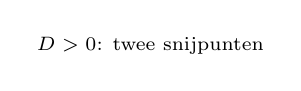
\begin{tikzpicture}[x=.32cm,y=.25cm]
  \roosterleeg{-3}{1}{3}{-3}{1}{5}
  \parabool{1}{0}{-2}{-2.65}{2.65}
  \punt{1.414}{0}\punt{-1.414}{0}
  \node[font=\scriptsize] at (0,-4.6) {$D > 0$: twee snijpunten};
\end{tikzpicture}\qquad
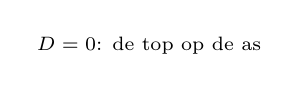
\begin{tikzpicture}[x=.32cm,y=.25cm]
  \roosterleeg{-3}{1}{3}{-3}{1}{5}
  \parabool{1}{0}{0}{-2.2}{2.2}
  \punt{0}{0}
  \node[font=\scriptsize] at (0,-4.6) {$D = 0$: de top op de as};
\end{tikzpicture}\qquad
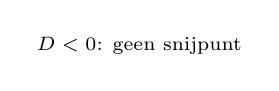
\begin{tikzpicture}[x=.32cm,y=.25cm]
  \roosterleeg{-3}{1}{3}{-3}{1}{5}
  \parabool{1}{0}{1.5}{-1.85}{1.85}
  \node[font=\scriptsize] at (0,-4.6) {$D < 0$: geen snijpunt};
\end{tikzpicture}}

\subsection{De formule gebruiken}

\voorbeeld{}{Los op: $2x^2 + 3x - 2 = 0$.\label{vb:h3-D}}{%
\uitleg{We lezen $a$, $b$ en $c$ af met hun teken, berekenen de discriminant en vullen de formule in.}
\begin{stappen}
a = 2,\ b = 3,\ c = -2 & \\
D = 3^2 - 4 \cdot 2 \cdot (-2) = 9 + 16 = 25 & $D > 0$: twee oplossingen. \\[1ex]
x_1 = \dfrac{-3 + 5}{4} = \dfrac12, \quad x_2 = \dfrac{-3 - 5}{4} = -2 & $\sqrt{25} = 5$ en $2a = 4$.
\end{stappen}
$V = \bigl\{-2, \tfrac12\bigr\}$. Controle: $2 \cdot 4 - 6 - 2 = 0$.}

\voorbeeld{}{Los op: $x^2 + 2x + 5 = 0$.\label{vb:h3-Dneg}}{%
\naast{\uitleg{Ook hier berekenen we eerst de discriminant.}
\begin{stappenvrij}{4.4cm}{4.1cm}
D = 2^2 - 4 \cdot 1 \cdot 5 = -16 & $D < 0$. \\
V = \emptyset & Geen oplossingen.
\end{stappenvrij}
\textit{De top van $y = x^2 + 2x + 5$ is $(-1, 4)$: ze ligt boven de $x$-as, en de parabool is naar boven geopend.}}{\begin{tikzpicture}[x=.4cm,y=.25cm]
  \rooster{-4}{1}{2}{-1}{1}{8}
  \parabool{1}{-1}{4}{-3}{1}
  \toppunt[below]{-1}{4}{}
\end{tikzpicture}}}

\begin{werkwijze}
Herleid de vergelijking tot $ax^2 + bx + c = 0$. Lees $a$, $b$ en $c$ af, met hun teken. Bereken $D = b^2 - 4ac$. Is $D < 0$, dan zijn er geen oplossingen. Is $D = 0$, dan is $x = -\tfrac{b}{2a}$. Is $D > 0$, vul dan $\sqrt D$ in de formule in, één keer met $+$ en één keer met $-$.
\end{werkwijze}

Welke methode kies je? Is $b = 0$, los dan op zoals $x^2 = k$. Is $c = 0$, breng dan $x$ buiten haakjes. Zie je snel een ontbinding, gebruik dan de product-nulregel. In alle andere gevallen werkt de discriminant. Die werkt trouwens ook in de eenvoudige gevallen, maar dan is ze trager.

\begin{oefeningen}
\oef{h3-discriminant}
\end{oefeningen}

\begin{alleenvoor}{4,5}
\subsection{Ontbinden met de oplossingen}

Ken je de oplossingen van $ax^2 + bx + c = 0$, dan ken je ook een ontbinding. Bij $x^2 - x - 12$ waren de oplossingen $-3$ en $4$, en de ontbinding $(x + 3)(x - 4)$. Bij $2x^2 + 3x - 2$ zijn de oplossingen $\tfrac12$ en $-2$. Is de ontbinding dan $(x - \tfrac12)(x + 2)$? Werk uit: $x^2 + \tfrac32 x - 1$. Dat is de helft van wat we zoeken: er moet nog een factor $a = 2$ voor.

\begin{theorie}
\begin{stelling}{Ontbinden met de oplossingen}
Heeft $ax^2 + bx + c = 0$ de oplossingen $x_1$ en $x_2$, dan is

\qquad $\formule{ax^2 + bx + c = a(x - x_1)(x - x_2)}$.

Is $D = 0$, dan is $x_1 = x_2$ en is $ax^2 + bx + c = a(x - x_1)^2$. Is $D < 0$, dan bestaat er geen ontbinding in factoren van de eerste graad.
\end{stelling}
\alleenvoor{5}{\begin{bewijs}
In hoofdstuk 2 vonden we met kwadraatafsplitsen dat $ax^2 + bx + c = a\bigl(x + \tfrac{b}{2a}\bigr)^2 + \tfrac{4ac - b^2}{4a}$, dus
\bewijsregel{ax^2 + bx + c = a\Bigl(\Bigl(x + \frac{b}{2a}\Bigr)^2 - \frac{D}{4a^2}\Bigr).}
Is $D \geqslant 0$, dan is $\tfrac{D}{4a^2} = \bigl(\tfrac{\sqrt D}{2a}\bigr)^2$, en met $A^2 - B^2 = (A - B)(A + B)$ is
\bewijsregel{ax^2 + bx + c = a\Bigl(x + \frac{b}{2a} - \frac{\sqrt D}{2a}\Bigr)\Bigl(x + \frac{b}{2a} + \frac{\sqrt D}{2a}\Bigr)}
\bewijsregel{\phantom{ax^2 + bx + c} = a\Bigl(x - \frac{-b + \sqrt D}{2a}\Bigr)\Bigl(x - \frac{-b - \sqrt D}{2a}\Bigr) = a(x - x_1)(x - x_2).}
Is $D < 0$ en zou $ax^2 + bx + c = a(x - r)(x - s)$ zijn, dan was $r$ een oplossing van $ax^2 + bx + c = 0$, volgens de product-nulregel. Maar er zijn geen oplossingen: zo'n ontbinding bestaat dus niet.
\end{bewijs}}
\end{theorie}

\alleenvoor{4}{Waarom klopt dat? In hoofdstuk 2 schreef je $ax^2 + bx + c$ met kwadraatafsplitsen als $a$ maal een verschil van twee kwadraten, $\bigl(x + \tfrac{b}{2a}\bigr)^2 - \tfrac{D}{4a^2}$. Met het merkwaardig product $A^2 - B^2 = (A - B)(A + B)$ wordt dat een product van twee factoren, en die zijn nul in $x_1$ en in $x_2$. Is $D < 0$, dan lukt dat niet: een factor $x - r$ zou een oplossing $r$ geven, en die zijn er niet.}

\voorbeeld{}{Ontbind $2x^2 + 3x - 2$ in factoren.\label{vb:h3-ontbindwortels}}{%
\uitleg{In voorbeeld~\ref{vb:h3-D} vonden we de oplossingen $\tfrac12$ en $-2$.}
\begin{stappen}
2x^2 + 3x - 2 = 2\Bigl(x - \frac12\Bigr)(x + 2) & $a = 2$, $x_1 = \tfrac12$, $x_2 = -2$. \\
= (2x - 1)(x + 2) & Breng de factor $2$ in de eerste haakjes.
\end{stappen}
Controle: $(2x - 1)(x + 2) = 2x^2 + 4x - x - 2 = 2x^2 + 3x - 2$.}

\begin{oefeningen}
\oef{h3-ontbindwortels}
\end{oefeningen}
\end{alleenvoor}

\begin{alleenvoor}{5}
\subsection{Som en product van de oplossingen}

Bij de som-productmethode zagen we dat $x^2 + bx + c$ met oplossingen $-m$ en $-n$ de som $m + n = b$ en het product $mn = c$ had. Dat verband tussen de oplossingen en de getallen in de vergelijking bestaat ook als $a \neq 1$.

\begin{theorie}
\begin{stelling}{Som en product}
Heeft $ax^2 + bx + c = 0$ de oplossingen $x_1$ en $x_2$ (met $D \geqslant 0$), dan is

\qquad $\formule{x_1 + x_2 = -\dfrac ba}$ \qquad en \qquad $\formule{x_1 \cdot x_2 = \dfrac ca}$.
\end{stelling}
\begin{bewijs}
Tel de twee formules op en vermenigvuldig ze:
\bewijsregel{x_1 + x_2 = \frac{-b + \sqrt D}{2a} + \frac{-b - \sqrt D}{2a} = \frac{-2b}{2a} = -\frac ba,}
\bewijsregel{x_1 \cdot x_2 = \frac{(-b + \sqrt D)(-b - \sqrt D)}{4a^2} = \frac{b^2 - D}{4a^2} = \frac{b^2 - b^2 + 4ac}{4a^2} = \frac ca.}
In het product gebruiken we het merkwaardig product $(A + B)(A - B) = A^2 - B^2$ met $A = -b$ en $B = \sqrt D$.

Voor de som kan het ook zonder rekenen, met de symmetrie. De oplossingen zijn de nulwaarden van $f(x) = ax^2 + bx + c$: twee punten van de parabool op hoogte $0$. Ze liggen dus symmetrisch om de as $x = -\tfrac{b}{2a}$ (hoofdstuk 1), en
\bewijsregel{\frac{x_1 + x_2}{2} = -\frac{b}{2a} \qquad\text{zodat}\qquad x_1 + x_2 = -\frac ba.}
\end{bewijs}
\end{theorie}

Zo controleer je snel een oplossing: bij $2x^2 + 3x - 2 = 0$ is $\tfrac12 + (-2) = -\tfrac32 = -\tfrac ba$ en $\tfrac12 \cdot (-2) = -1 = \tfrac ca$. Ken je één oplossing, dan vind je de andere zonder formule. Dat is vooral handig als $1$ of $-1$ een oplossing is, want dat zie je zonder te rekenen: $x = 1$ is een oplossing als $a + b + c = 0$, en $x = -1$ als $a - b + c = 0$.

\voorbeeld{}{Los op: $3x^2 - 5x + 2 = 0$.\label{vb:h3-eenoplossing}}{%
\uitleg{De som van de getallen is $3 - 5 + 2 = 0$. Dan is $x = 1$ een oplossing, want $3 \cdot 1^2 - 5 \cdot 1 + 2 = 0$. De andere vinden we met het product.}
\begin{stappen}
x_1 = 1 & Want $a + b + c = 0$. \\
1 \cdot x_2 = \dfrac ca = \dfrac23 & Het product van de oplossingen. \\[1ex]
x_2 = \dfrac23 & $V = \bigl\{\tfrac23, 1\bigr\}$.
\end{stappen}
Controle met de som: $1 + \tfrac23 = \tfrac53$, en $-\tfrac ba = \tfrac53$.}

\begin{oefeningen}
\oef{h3-somproduct}
\end{oefeningen}
\end{alleenvoor}

\begin{alleenvoor}{5}
\subsection{Bikwadratische vergelijkingen}

Sommige vergelijkingen van een hogere graad los je op met wat je nu kent. In $x^4 - 5x^2 + 4 = 0$ komen alleen $x^4 = (x^2)^2$ en $x^2$ voor. Noem je $x^2 = t$, dan staat er een tweedegraadsvergelijking in $t$. Zo'n vergelijking $ax^4 + bx^2 + c = 0$ heet \textit{bikwadratisch}.

\voorbeeld{}{Los op: $x^4 - 5x^2 + 4 = 0$.\label{vb:h3-bikwadratisch}}{%
\uitleg{We stellen $t = x^2$ en lossen op naar $t$. Daarna zoeken we bij elke $t$ de getallen $x$ met $x^2 = t$.}
\begin{stappen}
t^2 - 5t + 4 = 0 & Stel $t = x^2$, dan is $x^4 = t^2$. \\
(t - 1)(t - 4) = 0 & Product $4$, som $-5$. \\
t = 1 \ \text{ of } \ t = 4 & \\
x^2 = 1 \ \text{ of } \ x^2 = 4 & Terug naar $x$. \\
x = \pm 1 \ \text{ of } \ x = \pm 2 & $V = \{-2, -1, 1, 2\}$.
\end{stappen}
Een negatieve $t$ geeft geen oplossing. Bij $x^4 + 3x^2 - 4 = 0$ vind je $t = 1$ of $t = -4$, en $x^2 = -4$ kan niet. Daar is $V = \{-1, 1\}$.}

\begin{werkwijze}
Stel $t = x^2$ en los $at^2 + bt + c = 0$ op. Houd alleen de oplossingen $t \geqslant 0$ over, en los telkens $x^2 = t$ op. Zo heeft een bikwadratische vergelijking vier, drie, twee, één of geen oplossingen. Dezelfde substitutie werkt als een andere uitdrukking twee keer voorkomt, zoals $x^2 + x$ in $(x^2 + x)^2 - 8(x^2 + x) + 12 = 0$.
\end{werkwijze}

\begin{oefeningen}
\oef{h3-bikwadratisch}
\end{oefeningen}
\end{alleenvoor}

%========================================================================================
\section{Grafisch oplossen}

Elke tweedegraadsvergelijking kun je ook op een grafiek bekijken. Bij $f(x) = 0$ zoek je de snijpunten met de $x$-as. Bij $f(x) = k$ zoek je de snijpunten met de horizontale rechte $y = k$, zoals in het handboek Functies. En bij $f(x) = g(x)$, met $g$ een eerstegraadsfunctie, zoek je de snijpunten van een parabool en een rechte. Op de grafiek zie je hoeveel oplossingen er zijn en waar ze ongeveer liggen. De algebra geeft de exacte waarden.

\voorbeeld{}{Bepaal de snijpunten van de parabool $y = x^2$ en de rechte $y = x + 2$, grafisch en algebraïsch.\label{vb:h3-snijpunten}}{%
\naast{\uitleg{Op de grafiek lezen we twee snijpunten af. Algebraïsch zoeken we de $x$ waarvoor beide voorschriften dezelfde $y$ geven.}
\begin{stappenvrij}{3.6cm}{4.8cm}
x^2 = x + 2 & Dezelfde $y$-waarde. \\
x^2 - x - 2 = 0 & Herleid op nul. \\
(x - 2)(x + 1) = 0 & Product $-2$, som $-1$. \\
x = 2 \ \text{ of } \ x = -1 & \\
(2, 4) \text{ en } (-1, 1) & De $y$-waarden: vul in.
\end{stappenvrij}
\textit{De algebra bevestigt wat we op de grafiek aflezen.}}{\begin{tikzpicture}[x=.6cm,y=.4cm]
  \rooster{-3}{1}{3}{-1}{1}{6}
  \parabool{1}{0}{0}{-2.45}{2.45}
  \rechte[inkt]{-3}{3}{1}{2}
  \punt{2}{4}\punt{-1}{1}
  \aflezen{2}{4}\aflezen{-1}{1}
\end{tikzpicture}}}

\begin{oefeningen}
\oef{h3-grafisch}
\end{oefeningen}

%========================================================================================
\section{Vraagstukken}

Veel problemen leiden tot een tweedegraadsvergelijking: een oppervlakte, een baan of een prijs. De vergelijking heeft vaak twee oplossingen, terwijl het probleem er maar één heeft. Dan kijk je welke oplossing zin heeft.

\begin{werkwijze}
Kies wat je de onbekende noemt, met de eenheid. Schrijf de gegevens als een vergelijking. Herleid tot $ax^2 + bx + c = 0$ en los op. Kijk welke oplossingen zin hebben in het probleem, controleer met de gegevens, en antwoord in een zin.
\end{werkwijze}

\voorbeeld{}{Waar komt het water van de fontein uit hoofdstuk 2 in de vijver? De straal volgt $h(x) = -0,8x^2 + 3,2x + 0,4$.\label{vb:h3-fontein}}{%
\naast{\uitleg{Het water raakt de vijver als $h(x) = 0$. Om met kleinere getallen te werken, delen we eerst beide leden door $-0,8$.}
\begin{stappenvrij}{4cm}{4.3cm}
-0,8x^2 + 3,2x + 0,4 = 0 & \\
x^2 - 4x - 0,5 = 0 & Deel door $-0,8$. \\
D = 16 + 2 = 18 & $D > 0$. \\[1ex]
x = \dfrac{4 \pm \sqrt{18}}{2} & \\[1ex]
x \approx 4,12 \ \text{ of } \ x \approx -0,12 & $\sqrt{18} \approx 4,243$.
\end{stappenvrij}}{\begin{tikzpicture}[x=.55cm,y=.55cm]
  \fill[accent!12] (-.6,-.5) rectangle (5,0);
  \roosterleeg[$x$][$h$]{0}{1}{4.5}{0}{1}{4}
  \xgetallen{1,2,3,4}\ygetallen{1,2,3,4}
  \parabool{-.8}{2}{3.6}{0}{4.12}
  \punt{4.12}{0}
\end{tikzpicture}}
De oplossing $-0,12$ ligt achter de spuitmond: daar spuit de fontein niet. Het water komt op ongeveer $4,12$ m van de spuitmond in de vijver.}

\begin{oefeningen}
\oef{h3-vraagstuk}
\end{oefeningen}

\subsection{De top uit de nulwaarden}

In hoofdstuk 1 zag je dat de symmetrieas midden tussen de nulwaarden ligt. Staat het voorschrift als een product, dan lees je de nulwaarden af met de product-nulregel, en de top volgt met weinig rekenwerk. Je hoeft de haakjes niet uit te werken.

\voorbeeld{}{Een voetballer trapt een bal weg. Op een horizontale afstand $x$ (in m) is de bal $h(x) = -0,02x(x - 50)$ meter hoog. Hoe hoog komt de bal?\label{vb:h3-symnul}}{%
\naast{\uitleg{Het voorschrift is een product. De nulwaarden lezen we zo af, en de top ligt midden ertussen.}
\begin{stappenvrij}{4.4cm}{4cm}
x = 0 \ \text{ of } \ x = 50 & De nulwaarden, met de product-nulregel. \\[1ex]
x = \dfrac{0 + 50}{2} = 25 & De symmetrieas. \\[1ex]
h(25) = -0,02 \cdot 25 \cdot (-25) = 12,5 & De top is $(25;\ 12,5)$.
\end{stappenvrij}
\textit{De bal komt $12,5$ m hoog, na $25$ m. Zo werkt het ook bij $f(x) = (3x + 6)(2x - 1)$: de nulwaarden zijn $-2$ en $\tfrac12$, en de as ligt bij $x = \tfrac12\bigl(-2 + \tfrac12\bigr) = -\tfrac34$.}}{\begin{tikzpicture}[x=.08cm,y=.22cm]
  \roosterleeg[$x$][$h$]{0}{10}{55}{0}{5}{15}
  \xgetallen{10,20,30,40,50}\ygetallen{5,10}
  \symas{25}{0}{12.5}
  \parabool{-.02}{25}{12.5}{0}{50}
  \toppunt[above]{25}{12.5}{}
  \punt{0}{0}\punt{50}{0}
\end{tikzpicture}}}

\begin{oefeningen}
\oef{h3-symnul}
\end{oefeningen}

\voorbeeld{}{Terug naar het probleem. Het grasveld is $20$ m op $15$ m, en er is grind voor $200$ m$^2$. Hoe breed wordt het pad?\label{vb:h3-terug}}{%
\uitleg{Noem de breedte van het pad $x$ (in m). Grasveld en pad samen vormen een rechthoek van $20 + 2x$ op $15 + 2x$. Het pad is die rechthoek min het gras.}
\begin{stappenbreed}
(20 + 2x)(15 + 2x) - 300 = 200 & De oppervlakte van het pad. \\
300 + 40x + 30x + 4x^2 - 300 = 200 & Haakjes uitwerken. \\
4x^2 + 70x - 200 = 0 & Herleid op nul. \\
2x^2 + 35x - 100 = 0 & Deel door $2$: kleinere getallen. \\
D = 35^2 - 4 \cdot 2 \cdot (-100) = 1225 + 800 = 2025 & $\sqrt{2025} = 45$. \\[1ex]
x = \dfrac{-35 + 45}{4} = 2,5 \quad\text{of}\quad x = \dfrac{-35 - 45}{4} = -20 & Een breedte is positief.
\end{stappenbreed}
Het pad wordt $2,5$ m breed. Controle: $(20 + 5)(15 + 5) - 300 = 500 - 300 = 200$ m$^2$. Dat ligt inderdaad tussen de $156$ en $246$ m$^2$ die we vonden door te proberen.}

%========================================================================================
\opdrachtenkop

\begin{oefeningen}
\needspace{6\baselineskip}
\oef{h3-o1}

\needspace{6\baselineskip}
\oef{h3-o2}

\needspace{6\baselineskip}
\oef{h3-o24}

\needspace{6\baselineskip}
\oef{h3-o3}

\needspace{6\baselineskip}
\oef{h3-o5}

\needspace{6\baselineskip}
\oef{h3-o4}

\needspace{6\baselineskip}
\oef{h3-o6}

\needspace{6\baselineskip}
\oef{h3-o10}

\needspace{6\baselineskip}
\oef{h3-o7}


\needspace{6\baselineskip}
\oef{h3-o29}

\needspace{6\baselineskip}
\oef{h3-o11}

\needspace{6\baselineskip}
\oef{h3-o8}

\needspace{6\baselineskip}
\oef{h3-o21}

\needspace{6\baselineskip}
\oef{h3-o12}

\needspace{6\baselineskip}
\oef{h3-o9}

\needspace{6\baselineskip}
\oef{h3-o14}

\needspace{6\baselineskip}
\oef{h3-o15}

\needspace{6\baselineskip}
\oef{h3-o25}

\needspace{6\baselineskip}
\oef{h3-o16}


\needspace{6\baselineskip}
\oef{h3-o30}

\needspace{6\baselineskip}
\oef{h3-o13}

\needspace{6\baselineskip}
\oef{h3-o17}

\needspace{6\baselineskip}
\oef{h3-o19}


\needspace{6\baselineskip}
\oef{h3-o31}

\needspace{6\baselineskip}
\oef{h3-o18}

\needspace{6\baselineskip}
\oef{h3-o20}

\needspace{6\baselineskip}
\oef{h3-o22}

\needspace{6\baselineskip}
\oef{h3-o23}


\needspace{6\baselineskip}
\oef{h3-o26}


\needspace{6\baselineskip}
\oef{h3-o27}


\needspace{6\baselineskip}
\oef{h3-o28}


\needspace{6\baselineskip}
\oef{h3-o32}
\end{oefeningen}

%----------------------------------------------------------------------------------------
\needspace{14\baselineskip}
\opdrachtsectie{Test jezelf}

\begin{oefeningen}
\needspace{6\baselineskip}
\oef{h3-t1}

\needspace{6\baselineskip}
\oef{h3-t2}

\needspace{6\baselineskip}
\oef{h3-t3}

\needspace{6\baselineskip}
\oef{h3-t4}

\needspace{6\baselineskip}
\oef{h3-t5}

\needspace{6\baselineskip}
\oef{h3-t6}

\needspace{6\baselineskip}
\oef{h3-t7}

\needspace{6\baselineskip}
\oef{h3-t8}

\needspace{6\baselineskip}
\oef{h3-t9}
\end{oefeningen}

\herhaalschema{%
  \fv{oef:h3-t1}{vb:h3-zonderc}{oef:h3-onvolledig}%
  \fv{oef:h3-t2}{vb:h3-somproduct}{oef:h3-ontbinden}%
  \fv{oef:h3-t3}{vb:h3-D}{oef:h3-discriminant}%
  \fv{oef:h3-t4}{vb:h3-Dneg}{oef:h3-o5}%
  \fv{oef:h3-t5}{vb:h3-herleid}{oef:h3-nul}%
  \fv{oef:h3-t6}{vb:h3-snijpunten}{oef:h3-grafisch}%
  \fv{oef:h3-t7}{vb:h3-terug}{oef:h3-vraagstuk}%
  \alleenvoor{4,5}{\fv{oef:h3-t8}{vb:h3-ontbindwortels}{oef:h3-ontbindwortels}}%
  \alleenvoor{5}{\fv{oef:h3-t9}{vb:h3-bikwadratisch}{oef:h3-bikwadratisch}}}

\ifzelfstudie
\section*{Maak je eigen samenvatting}
Sluit dit boek en schrijf in je schrift: wat een tweedegraadsvergelijking is en wat de oplossingen op de grafiek betekenen, hoe je $ax^2 + c = 0$ en $ax^2 + bx = 0$ oplost, de product-nulregel en waarom je eerst op nul moet herleiden, de som-productmethode, de discriminant en de formule met haar drie gevallen\alleenvoor{4,5}{, hoe je ontbindt met de oplossingen}\alleenvoor{5}{, de som en het product van de oplossingen, hoe je een bikwadratische vergelijking oplost}, hoe je grafisch oplost, en hoe je een vraagstuk aanpakt. Vergelijk daarna met de kaders.
\fi
